\documentclass[onecolumn, 12pt]{book}

\usepackage[latin1]{inputenc}   
\usepackage{amsmath}
\usepackage{algorithm}
\usepackage{algorithmic} 
%\usepackage[T1]{fontenc}

%\usepackage[francais]{babel}     
\usepackage{layout}    
\usepackage[top=2cm, bottom=2cm, left=2cm, right=2cm]{geometry} 
\usepackage{setspace}
\usepackage{soul}
\usepackage{color} 
\usepackage{verbatim}
\usepackage{moreverb}
\usepackage{listings}
\usepackage{url}
\usepackage{graphicx}
%\usepackage{epstopdf}
%\usepackage[outdir=/home/willy/Documents/latexDoc/redaction/fusion_fichiers/images_fusionChapitres/]{epstopdf}
%\usepackage[outdir=./../../fusion_fichiers/images_fusionChapitres/]{epstopdf}
\usepackage[outdir=./]{epstopdf}
\usepackage{caption}
\usepackage{setspace}
\usepackage{enumitem} 
\usepackage{amsthm} % ajouter pour environnement proof
\usepackage{placeins}

 \newcounter{subsubsubsection}
\renewcommand\thesubsubsubsection{\thesubsubsection.\arabic{subsubsubsection}}
\renewcommand\theparagraph{\thesubsubsubsection.\arabic{paragraph}} % optional; useful if paragraphs are to be numbered
\setcounter{secnumdepth}{4}
\setcounter{tocdepth}{4}

\title{Chapitre6 : Exp\'erimentations sur des donn\'ees al\'eatoires}
\author{Wilfried Ehounou}
\date{\oldstylenums{\today}} 


%--- d\'efinition macro ------
\def\R{\mbox{I\hspace{-.15em}R}}
\def\N{\mbox{I\hspace{-.15em}N}}
\def\Z{\mbox{I\hspace{-.15em}Z}}
\def\Q{\mbox{I\hspace{-.15em}Q}}

\newtheorem{definition}{D\'efinition}
\newtheorem{theorem}{Th\'eor\`eme}
\newtheorem{property}{Propri\'et\'e}
\newtheorem{claim}[theorem]{Claim}
\newtheorem{proposition}[theorem]{Proposition}
\newtheorem{lemma}[theorem]{Lemma}
\newtheorem{corollary}[theorem]{Corollary}
\newtheorem{conjecture}[theorem]{Conjecture}
\newtheorem{observation}{Observation}
\newtheorem{example}{Exemple}
\newtheorem{remark}{Remarque}

%---- path figures ----
\graphicspath{
{/home/willy/Documents/latexDoc/redaction/fusion_fichiers/images_fusionChapitres/}
}
 
\begin{document}
	Les graphes cellules sont des graphes dans lesquels chaque sommet est couvert par plus de $2$ cliques. Ce qui implique la couverture de corr\'elation est vide parce que  le couverture des ar\^etes de cette famille de graphes  est impossible. Tous les sommets de ces graphes sont alors contenus dans l'ensemble ${\cal C}$ des sommets \`a corriger.
\newline
Dans cette section, nous montrons que la correction de ces graphes peut se r\'ealiser en ajoutant ou en supprimant des ar\^etes uniquement.
Nous consid\'erons deux fonctions de co\^ut {\em ajout} et {\em suppression} qui correspondent respectivement \`a l'ajout et la suppression d'ar\^etes pendant l'algorithme de correction. Puis nous v\'erifions si la correction des graphes cellules convergent vers les bornes sup\'erieures des distances line de chaque fonction. 
Pour ce faire, nous corrigeons les sommets de  ${\cal C}$ avec le mode {\em al\'eatoire sans remise} en utilisant les fonctions {\em ajout} et {\em suppression}.
\newline
Nous d\'ebutons notre analyse par la d\'efinition et la construction d'un graphe cellule. Ensuite, nous d\'ecrirons le protocole d'exp\'erimentation sur des graphes cellules d'ordres diff\'erents. Enfin nous interpr\'etons les r\'esultats obtenus pour chaque fonction de co\^ut.
	\subsection{D\'efinition des graphes cellules et les distances line th\'eoriques}
		Soit $G_{k,k'}$ la famille de graphes cellules dans laquelle $k$ et $k'$ d\'esignent le nombre de graphes cellules respectivement par lignes et colonnes.
Nous pr\'ecisons que les nombres $k$ et $k'$ sont {\em impairs}.

\begin{definition}
Une cellule est un graphe biparti $K_{2,2}$ non orient\'e avec un cycle.
\end{definition}

\begin{definition}
Le graphe $G_{1,1}$ est une cellule.
\end{definition}

% definir la cellule en fonction de n,m  n in k et m in k'
		\subsubsection{Construction du graphe cellule $G_{k,k'}$ }
			
Soient $n$ et $m$ deux entiers tels que $n < k$ et $m < k'$.
Consid\'erons une cellule $G_{n,m}$ qui contient $4$ sommets et $4$ ar\^etes.
Les sommets de  $G_{n,m}$  sont not\'es par les couples $(n,m)$, $(n,m+1)$, $(n+1,m)$,  $(n+1,m+1)$. 

% -----
Nous d\'esignons par 
\begin{itemize}
\item $e_{n} = \{(n,m),(n,m+1)\}$ l'ar\^ete entre les sommets $(n,m)$ et $(n,m+1)$,   
\item $e_{m} = \{(n,m),(n+1,m)\}$ l'ar\^ete entre les sommets $(n,m)$ et $(n+1,m)$,   
\item $e_{n+1} = \{(n+1,m),(n+1,m+1)\}$ l'ar\^ete entre les sommets $(n+1,m)$ et $(n+1,m+1)$,   
\item $e_{m+1} = \{(n,m+1),(n+1,m+1)\}$ l'ar\^ete entre les sommets $(n,m+1)$ et $(n+1,m+1)$.
\end{itemize}
Nous faisons varier $n$ et $m$ par pas de $1$ et nous s\'electionnons les cellules $G_{n,m}$ et $G_{n,m+1}$.
L'ar\^ete $e_{m+1}$ est commune aux cellules $G_{n,m}$ et $G_{n,m+1}$. 
De m\^eme, les cellules $G_{n,m}$ et $G_{n+1,m}$ partagent l'ar\^ete $e_{n+1}$. 
Ainsi, \`a chaque \'etape de la construction, chaque cellule partage 
$2$ ar\^etes si $n = m = 0$ ou $n = k-1 ~et~ m = k'-1$,
$3$ ar\^etes si $n = \{0,k-1\} ~et~ m \neq \{0,k'-1\}$ ou $m = \{0,k'-1\} ~et~ n \neq \{0,k-1\}$, 
$4$ ar\^etes si $n \neq \{0,k-1\} ~et~ m \neq \{0,k'-1\}$. 
\newline
\`A la fin de la boucle, nous ajoutons les ar\^etes $\{(0,0),(k+1,0)\}$, $\{(0,0),(0,k+1)\}$, $\{(k+1,k'+1),(k+1,0)\}$ et $\{(k+1,k'+1),(0,k+1)\}$.
Nous obtenons ainsi le graphe $G_{k,k'}$.
% -----

\begin{definition}
Le graphe $G_{k,k'}$ poss\`ede $(k+1) \times (k'+1)$ sommets,  $k \times (k'+1) + k' \times(k+1) + 4$  ar\^etes et $k \times k' +1$ cellules.
\end{definition}

% ---- figure exemple graphe cellule G_{3,3}
\begin{figure}[htb!] 
\centering
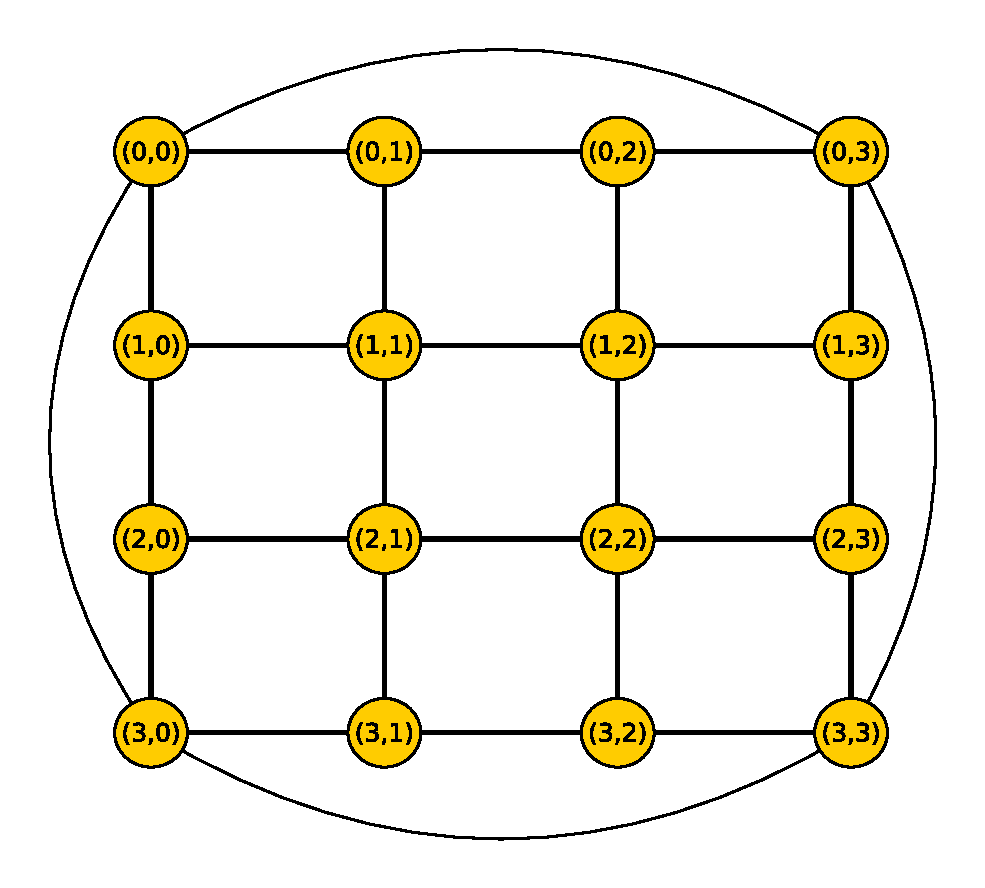
\includegraphics[scale=0.6]{exempleGrapheCelluleG33.eps}
\caption{ Le graphe cellule $G_{3,3}$ : il est compos\'e de $16$ sommets, $28$ ar\^etes et $9$ cellules. }
\label{exempleGrapheCellule} 
\end{figure}
%\FloatBarrier
% ---- figure exemple graphe cellule G_{3,3}

Dans la figure \ref{exempleGrapheCellule}, nous avons un exemple de graphe cellule $G_{3,3}$ avec $k=3$ et $k'=3$. Nous avons $16$ sommets, $28$ ar\^etes et $9$ cellules. 
		\subsubsection{Correction des graphes cellules}
			Le graphe cellule $G_{k,k'}$ ne contient aucune clique. 
Nous appliquons l'algorithme de correction pour cr\'eer des cliques qui couvrent les sommets de ${\cal C}$ et dont le line-graphe propos\'e est de distance minimale.
Pour effectuer la correction, nous pouvons soit ajouter ou soit supprimer des ar\^etes uniquement.
Soient la fonction de co\^ut {\em ajout} qui ajoute uniquement des ar\^etes et la fonction de co\^ut {\em suppression} qui supprime uniquement des ar\^etes. 
Nous allons d\'etailler les op\'erations d'ajout et de suppression d'ar\^etes pendant l'algorithme de correction. 

\subsubsection{Correction avec la fonction {\em ajout}}
Soit le graphe $G_{k,k'}$ contenant $k \times k' + 1$ cellules.
Pour transformer chaque cellule en cliques, nous devons ajouter $2$ ar\^etes.
Nous consid\'erons le sommet $(0,0)$ contenu dans les cellules $G_{0,0}$ et $G_{k,k'}$.
Nous ajoutons $2$ ar\^etes dans $G_{0,0}$ et $G_{k,k'}$. Les cellules deviennent des cliques $K_4$. 
\newline
L'ar\^ete $\{(0,1),(1,1)\}$ appartient aux cellules  $G_{0,0}$ et  $G_{0,1}$. Or cette ar\^ete est d\'ej\`a couverte par une clique $K_4$ de la cellule $G_{0,0}$. Alors nous ne pouvons pas ajouter d'ar\^etes dans la cellule $G_{0,1}$. L'ar\^ete $\{(0,1),(0,2)\}$ forme une clique $K_2$. Le sommet $(0,1)$ est couvert par une clique $K_4$ et une clique $K_2$. 
Le sommet $(1,0)$ est aussi couvert par une clique $K_4$ et une clique $K_2$ parce que les cellules $G_{0,0}$ et  $G_{1,0}$ partagent l'ar\^ete $\{(1,0),(1,1)\}$  et cette ar\^ete forme une clique $K_4$ avec la cellule $G_{0,0}$.
Les $G_{0,0}$ et  $G_{1,1}$ ne partagent que le sommet  $(1,1)$. En plus les ar\^etes  $\{(1,1),(2,1)\}$ de  $G_{1,0}$ et  $\{(1,1),(1,2)\}$ de $G_{0,1}$ ne sont pas couverts par une clique $K_4$. Nous pouvons alors transformer $G_{1,1}$ en une clique $K_4$  en ajoutant $2$ ar\^etes .
\newline
Ainsi, dans les cellules cons\'ecutives quelle que soit la ligne (avec $k$) et la colonne (avec $k'$), nous ajoutons des ar\^etes dans une cellule sur deux. 
%Une ar\^ete d'une cellule dans laquelle nous n'avons pas ajout\'e d'aretes devient une clique $K_2$. 
L'ar\^ete  d'une cellule qui n'est pas contenue par une clique $K_4$ forme une clique $K_2$.
Les cellules ayant un seul sommet en commun sont transform\'ees en des cliques $K_4$. 
\newline
\`A la fin  de la correction, le graphe cellule $G_{k,k'}$ est partitionn\'e par des cliques $K_4$ et $K_2$.
La distance de Hamming entre $G_{k,k'}$ et $L(G_{k,k'})$ est de $DH_{k,k'} = 2 \times (\lceil \frac{k \times k'}{2} \rceil  + 1)$ et cette distance est minimale.
\begin{theorem}
La distance line d'un graphe cellule $G_{k,k'}$ avec la fonction {\em ajout} est 
\begin{equation}
DL_{ajout}(G_{k,k'}) = 2 \times (\lceil \frac{k \times k'}{2} \rceil  + 1)
\end{equation}
\end{theorem}

% ---- figure exemple correction graphe cellule G_{3,3}
\begin{figure}[htb!] 
\centering
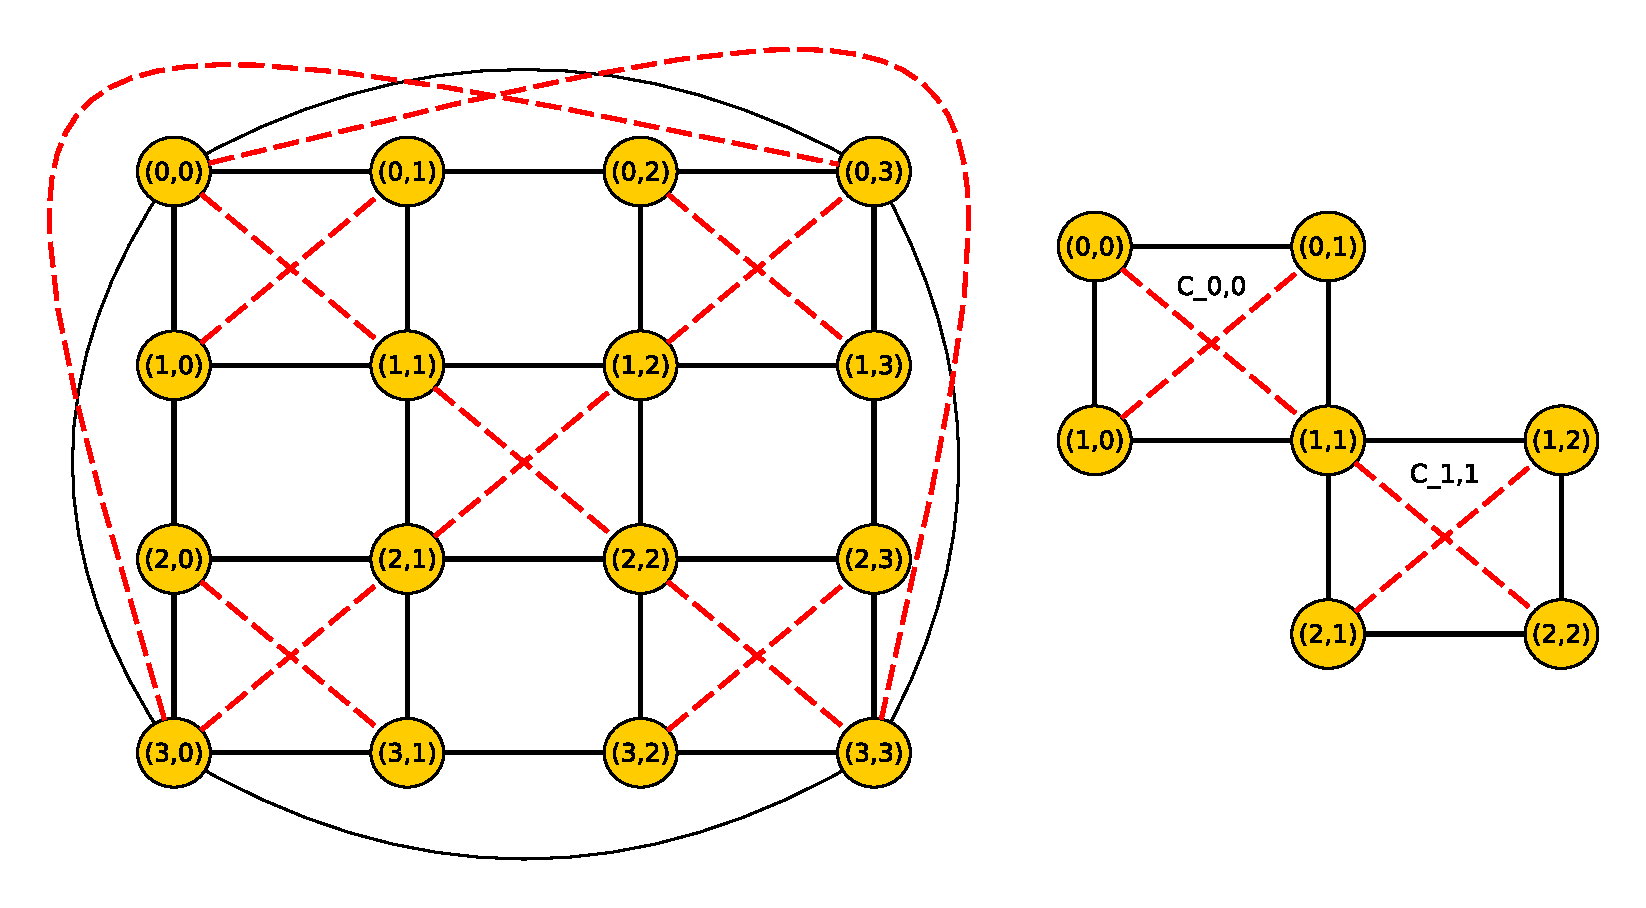
\includegraphics[scale= 0.7]{exempleGrapheCelluleAjoutG33.eps}
\caption{ Le graphe cellule $G_{3,3}$ : il est compos\'e de $16$ sommets, $33$ ar\^etes. Il contient $4$ cliques $K_{2}$ et $6$ cliques $K_4$. Les ar\^etes ajout\'ees sont les traits de couleur rouge.}
\label{exempleCorrectionGrapheCelluleAvecAjout}
\end{figure}
% ---- figure exemple correction graphe cellule G_{3,3}
Dans la figure \ref{exempleCorrectionGrapheCelluleAvecAjout}, nous r\'ealisons la correction de distance line minimale en transformant les cellules partageant un sommet en cliques $K_4$. C'est le cas des cellules $G_{1,2}$ et  $G_{0,2}$ qui ont le sommet $(1,2)$ en commun. 
Les ar\^etes partag\'ees entre deux cellules ont un des sommets couvert par une clique $K_2$ et l'autre sommet couvert par une clique $K_4$. Tel est le cas avec le sommet $(3,2)$ qui forme l'ar\^ete $\{(2,2),(3,2)\}$ et cette ar\^ete est contenue par une clique $K_4$.

\subsubsection{Correction avec la fonction {\em suppression}}
Soit le graphe $G_{k,k'}$ contenant $k \times k' + 1$ cellules.
Pour transformer chaque cellule en cliques, nous devons supprimer $3$ ar\^etes dans la cellule $G_{k,k'}$ et $1$ ar\^ete dans les autres cellules.
Nous consid\'erons un sommet  de degr\'e minimun par exemple$(0,1)$. Ce sommet appartient \`a $2$ cellules  $G_{0,0}$ et $G_{0,1}$. Pour que le sommet $(0,1)$ soit couvert par $2$ cliques de cellules diff\'erentes, nous supprimons l'ar\^ete $\{(0,1),(1,1)\}$ et nous formons ainsi $2$ cliques $K_2$ dans chacune des cellules. 
\newline
Ensuite, en consid\'erant les sommets de degr\'e minimum \`a chaque correction de sommet, nous supprimons les ar\^etes verticales dans chaque ligne. 
Par exemple, les ar\^etes $\{(0,3),(1,3)\}$ et $\{(0,4),(1,4)\}$ entre respectivement les cellules $G_{0,2}$ et  $G_{0,3}$ et  les cellules $G_{0,3}$ et  $G_{0,4}$ sont supprim\'ees. Ainsi les cellules de chaque ligne ne partagent aucune ar\^ete entre elles et chaque cellule ne contient que $2$ ar\^etes verticales. Ces $2$ ar\^etes forment $2$ cliques $K_2$.
\newline
Il nous reste que les sommets de degr\'e $4$. Les ar\^etes formant des cliques $K_2$  et incidentes \`a un tel sommet sont conserv\'ees et les autres ar\^etes sont supprim\'ees.  Par exemple, prenons le sommet $(0,0)$ qui est couvert par $2$ cliques $K_2$ ($\{(0,0),(1,0)\}$ et $\{(0,0),(0,1)\}$). Nous supprimons les ar\^etes  $\{(0,0),(0,k'+1)\}$ et $\{(0,0),(k+1,0)\}$).
\newline
Pour les sommets \'etant couverts par une clique $K_2$, nous supprimons les ar\^etes verticales des cellules dont ils appartiennent. Par exemple, en s\'electionnant le sommet $(0,k'+1)$, il est d\'ej\`a couvert par la clique $K_2 = \{(0,k'),(0,k'+1)\}$ et l'ar\^ete $\{(0,0),(0,k'+1)\}$ a d\'ej\`a \'et\'e supprim\'ee. Nous supprimons l'ar\^ete  $\{(0,k'+1), (1, k'+1)\}$ et le sommet  $(0,k'+1)$ est alors couvert par $2$ cliques $K_2$ ($\{(0,k'),(0,k'+1)\}$ et $(0,k'+1),(k+1,k'+1)$).
\newline
Cette op\'eration de correction est aussi correcte si nous supprimons les ar\^etes horizontales dans chaque colonne. 
\newline
\`A la fin de l'algorithme de correction, le graphe $G_{k,k'}$ est partitionn\'e avec des cliques $K_2$ et ce graphe est un cycle de taille $(k \times k'+1) + k' + 1$.
La distance de Hamming   entre $G_{k,k'}$ et $L(G_{k,k'})$ est $DH_{k,k'} = k \times k' +3 $ et cette distance est minimale.

\begin{theorem}
La distance line  d'un graphe cellule $G_{k,k'}$ avec la fonction {\em suppression} est 
\begin{equation}
DL_{supp}(G_{k,k'}) = k \times k' +3 
%DL_{supp}(G_{k,k'}) = k \times (k' +1) ===> cela correspond a quoi?
\end{equation}
\end{theorem}

% ---- figure exemple correction graphe cellule G_{3,3}
\begin{figure}[htb!] 
\centering
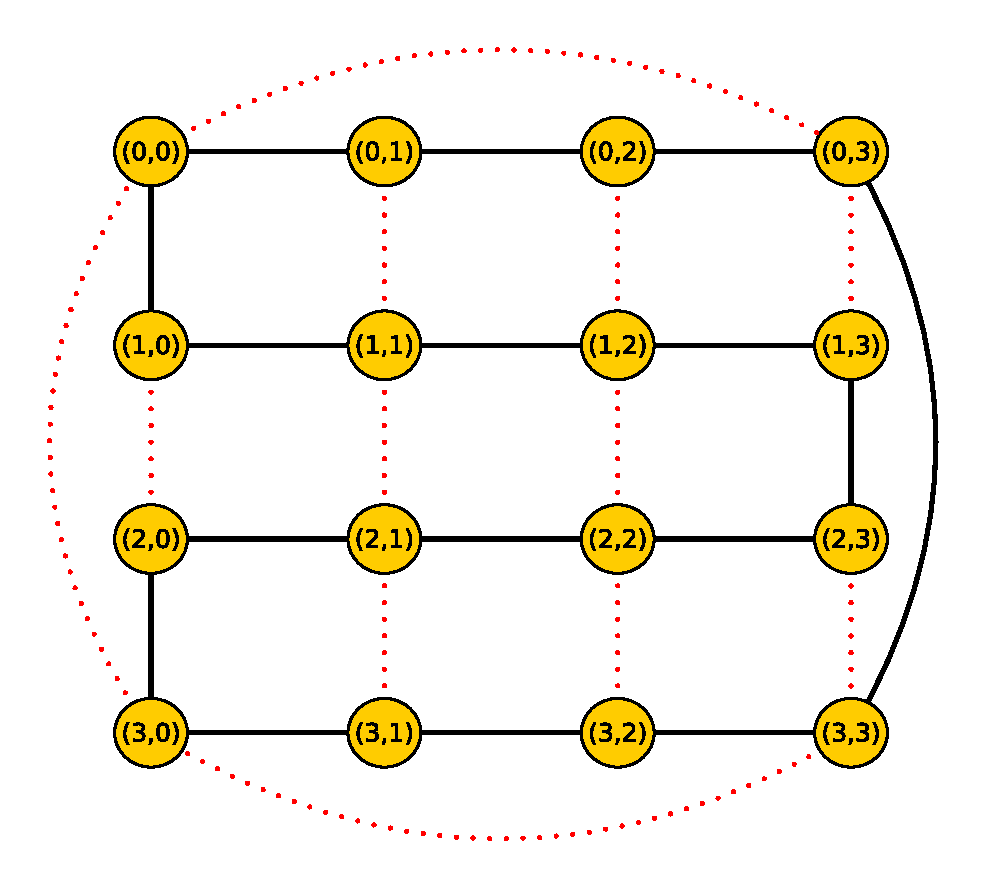
\includegraphics[scale = 0.7]{exempleGrapheCellulesSuppressionG33.eps}
\caption{ Le graphe cellule $G_{3,3}$ : il est compos\'e de $16$ sommets, $16$ ar\^etes et $16$ cliques $K_2$. Les ar\^etes supprim\'ees sont les traits en pointill\'ees rouges }
\label{exempleCorrectionGrapheCelluleAvecSuppression}
\end{figure}
% ---- figure exemple correction graphe cellule G_{3,3}
Une illustration de la correction avec la fonction suppression est faite avec le graphe $G_{3,3}$ dans la figure \ref{exempleCorrectionGrapheCelluleAvecSuppression}.
Le graphe $G_{3,3}$ poss\`ede $(k+1)\times (k'+1) = 16$ cliques $K_2$ et $12$ ar\^etes sont supprim\'ees.
\newline

% conclusion
Nous avons d\'etermin\'e les distances line th\'eoriques selon les fonctions de co\^ut lors de la correction de sommets de graphes cellules. Nous allons v\'erifier si les distances line obtenues exp\'erimentalement convergent vers les distances line th\'eoriques.






	\subsection{Protocole d'exp\'erimentation sur les graphes Iourtes}
		Consid\'erons $G_{k,k'}$ un graphe cellule dans lequel le nombre de lignes est identique le nombre de colonnes ($k = k'$). Nous notons $G_k$ pour d\'esigner $G_{k,k'}$ et $G_k$ contient $k \times k +1$ cellules.
Nous construisons $48$ graphes cellules dans lesquels chaque graphe contient $k \times k +1$ cellules $k \in \{1,3,\cdots,99\}$.
Dans chaque graphe $G_k$, nous ex\'ecutons  notre couple d'algorithmes $50$ fois puis nous r\'ecup\'erons la distance line  minimale entre $G_k$ et les line-graphes $L(G_k)$ propos\'ees.
Nous utilisons la   distance line  minimale parce qu'il est impossible de trouver la bonne permutation qui minimise la distance line \`a cause de la combinatoire factorielle de l'ensemble $\cal C$.
\newline
Soient $\phi^{+}(u,v)$ le poids de l'op\'eration {\em ajouter une ar\^ete} et $\phi^{-}(u,v)$ le poids de l'op\'eration {\em supprimer une ar\^ete}. 
Nous d\'efinissons les fonctions de co\^ut {\em ajout} et {\em suppression} comme suit :
\begin{enumerate}[label = (\alph*)]
%\item {\em unitaire} : ajouter et supprimer une ar\^ete ont un poids $1$ ($\phi^{+} = \phi^{-} = 1$).
\item {\em ajout} : nous donnons un poids minimal \`a l'op\'eration ``ajouter d'ar\^etes''. Ainsi nous attribuons un poids $\phi^{+} = 1$ pour l'ajout d'ar\^etes et un poids $\phi^{-} = 10$ pour la suppression d'ar\^etes.
\item {\em suppression} : Ici nous faisons l'op\'eration inverse en donnant un poids maximal \`a l'op\'eration d'ajout d'ar\^etes. Ainsi, l'ajout d'une ar\^ete a un poids $\phi^{+} = 10$ alors que la suppression a un poids $\phi^{-} = 1$.
\end{enumerate}
L'objectif de notre exp\'erimentation est de comparer les distances lines th\'eoriques avec celles obtenus avec l'utilisation des fonctions de co\^uts mentionn\'ees ci-dessus.


%Nous allons comparer les diff\'erentes fonctions de co\^ut en utilisant les distances line calcul\'ees. Les courbes croissantes dans les figures \ref{priorAjout1Ajout10}, \ref{priorAjout1Supp10} et \ref{priorAjout1Supp1} s'explique par le fait que les distances line sont rang\'ees par ordre croissant.
	\subsection{Analyse des r\'esultats}
		% ---- figure comparaison_distances_line_graphes_cellules_k_2x50
\begin{figure}[htb!] 
\centering
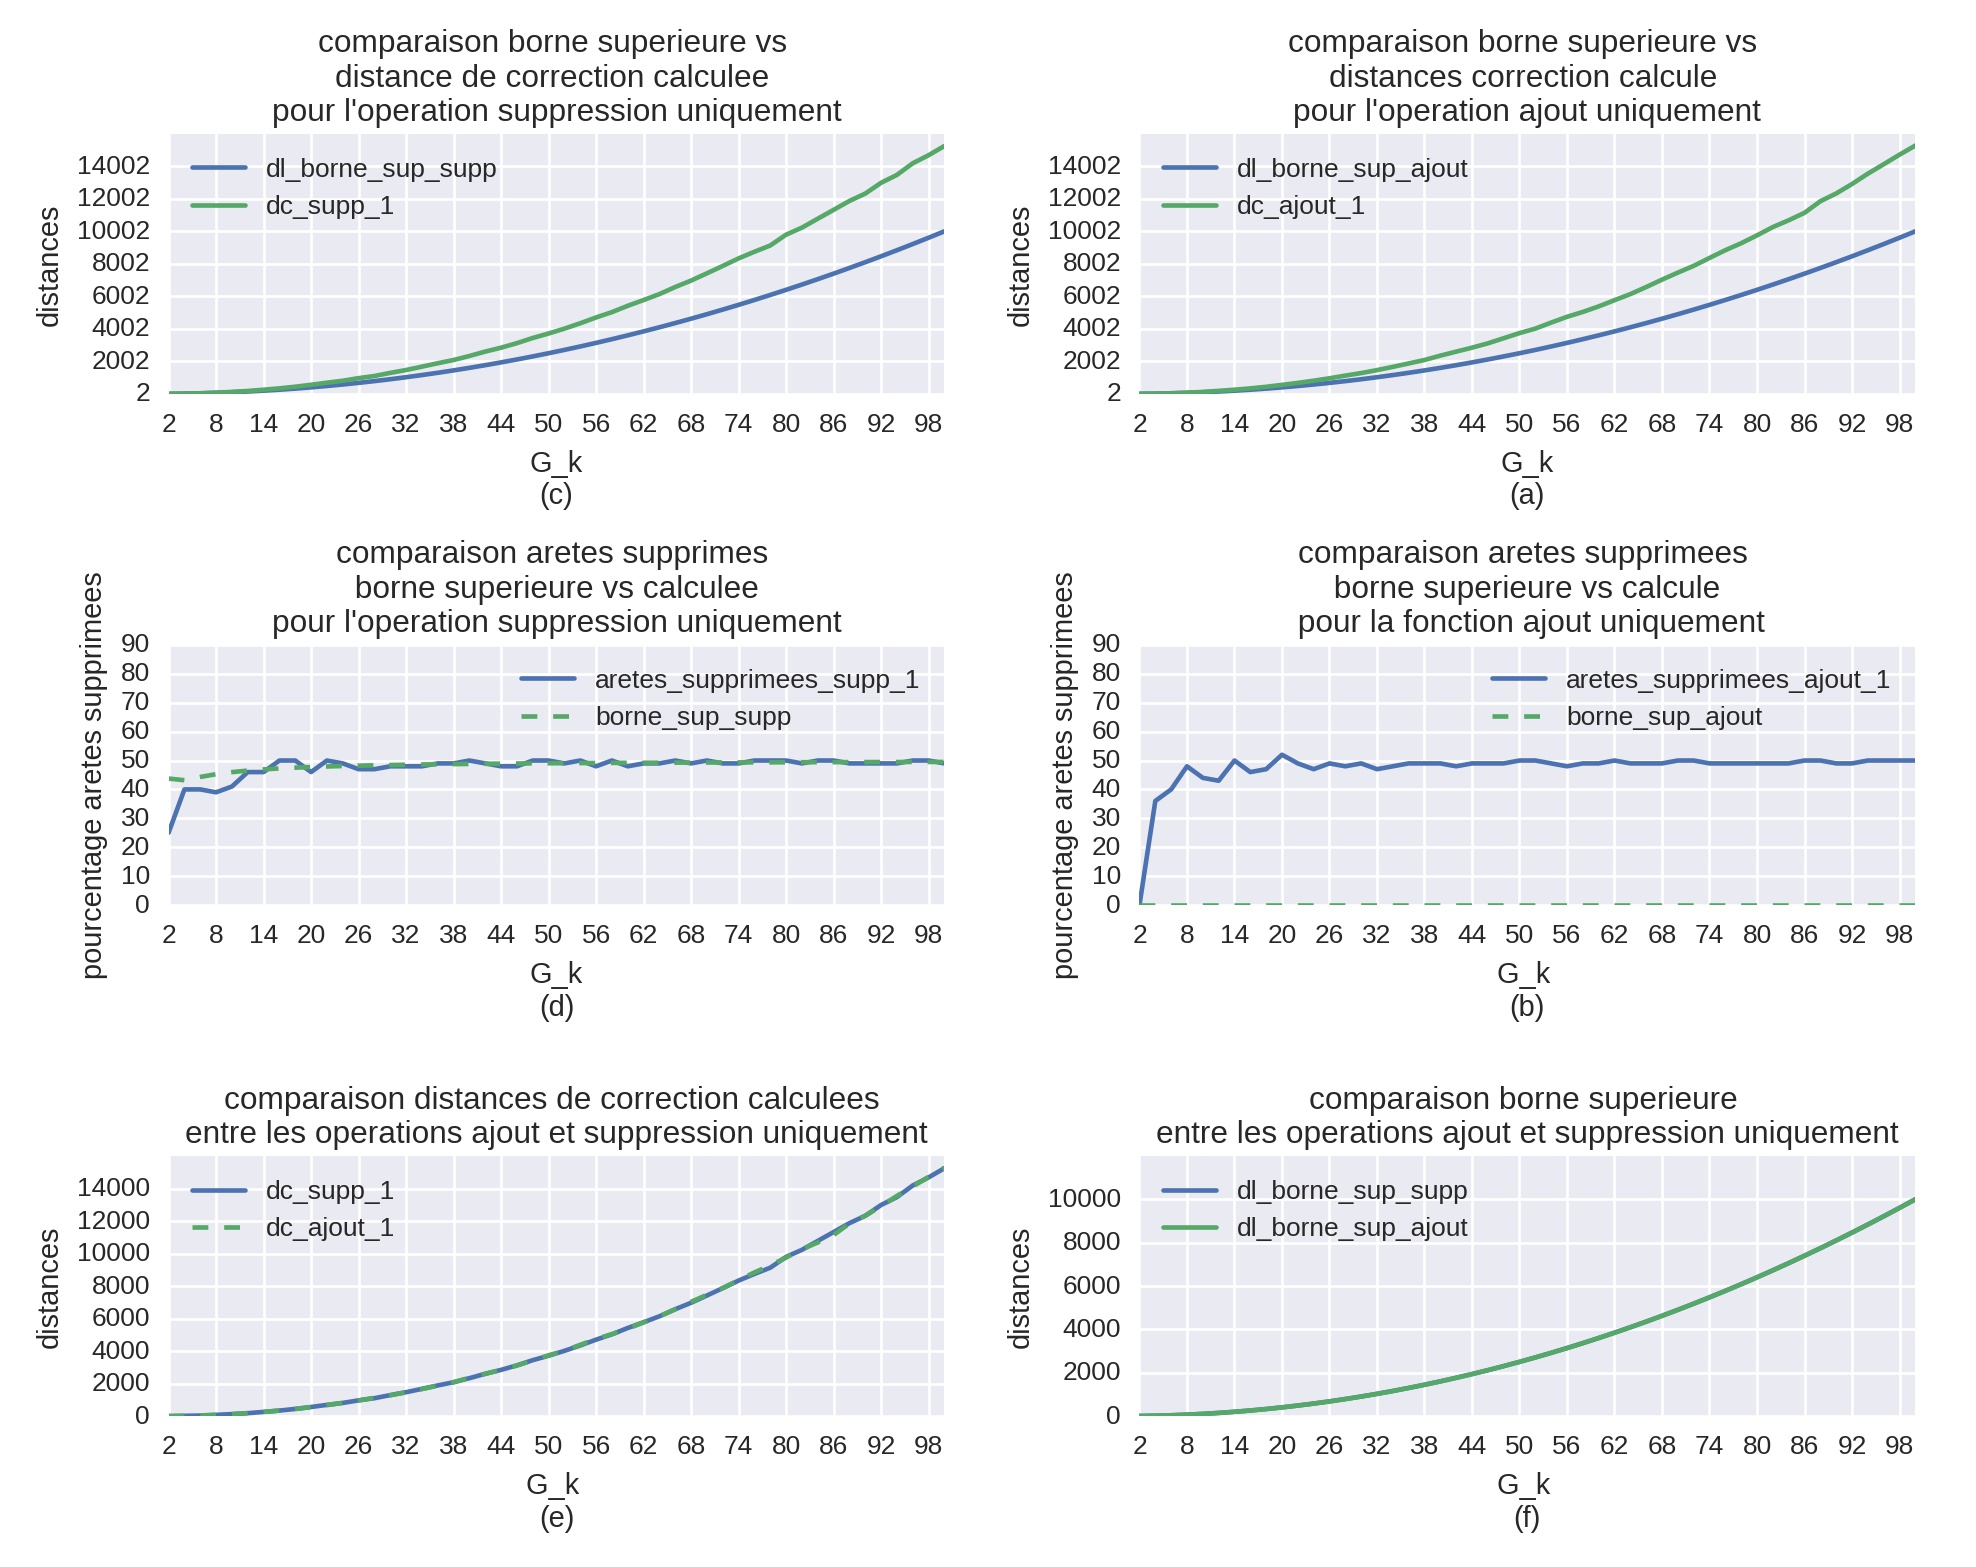
\includegraphics[scale = 0.25]{comparaison_distances_line_graphes_cellules_k_2x50.jpeg}
\caption{Comparaison des distances lines th\'eoriques et calcul\'ees selon des fonctions de co\^ut {\em suppression} et  {\em ajout}.
La figure $(a)$ d\'esigne la comparaison de distances line pour la fonction {\em ajout} entre les distances th\'eoriques et celles obtenues apr\`es l'ex\'ecution de l'algorithme de correction. 
La figure $(b)$ repr\'esente la comparaison entre les ar\^etes supprim\'ees th\'eoriques et celles obtenues apr\`es la correction pour la fonction {\em ajout}.
La figure $(c)$ repr\'esente la comparaison entre les distances line th\'eoriques et celles obtenues apr\`es la correction pour la fonction {\em ajout}.
La figure $(d)$ repr\'esente la comparaison entre les ar\^etes supprim\'ees th\'eoriques et celles obtenues apr\`es la correction pour la fonction {\em suppression}.
La figure $(e)$ repr\'esente la comparaison des distances line obtenues apr\`es l'ex\'ecution de l'algorithme de correction entre les fonctions {\em suppression} et {\em ajout}.
La figure $(f)$ repr\'esente la comparaison des distances line th\'eoriques entre les fonctions {\em suppression} et {\em ajout}.
}
\label{comparaison_distances_line_graphes_cellules_k_2x50}
\end{figure}
% ---- figure comparaison_distances_line_graphes_cellules_k_2x50

Nous r\'ealisons cinq comparaisons et les r\'esultats obtenus sont regroup\'es en $6$ exp\'erimentations.
\newline
Les deux premi\`eres exp\'erimentations comparent les distances line th\'eoriques et celle obtenues apr\`es l'ex\'ecution de nos algorithmes pour chaque fonction de co\^ut. Le terme {\em th\'eorique} signifie que le line-graphe obtenu apr\'es la correction du graphe cellule $G_k$ est optimal c'est-\`a-dire la distance line de $G_k$ est minimale. 
La figure \ref{comparaison_distances_line_graphes_cellules_k_2x50}(c) d\'esigne la comparaison avec la fonction {\em suppression} entre la distance line th\'eorique {\em dl\_theorique\_supp} et la distance line calcul\'ee {\em dl\_supp\_1}. Alors que la fonction {\em ajout} est repr\'esent\'ee par la figure \ref{comparaison_distances_line_graphes_cellules_k_2x50}(a) dans laquelle nous comparons les distances line th\'eoriques {\em dl\_theorique\_ajout}  et calcul\'ees {\em dl\_ajout\_1}.  

Les  exp\'erimentations  des figures \ref{comparaison_distances_line_graphes_cellules_k_2x50}$(d)$ et \ref{comparaison_distances_line_graphes_cellules_k_2x50}$(b)$ indiquent, respectivement, le pourcentage d'ar\^etes supprim\'ees dans les graphes $G_k$ pour les fonctions de co\^ut {\em suppression} et {\em ajout}. Nous avons determin\'e th\'eoriquement le nombre d'ar\^etes \`a supprimer pour obtenir le line-graphe optimal et nous comparons ce nombre avec celui des ar\^etes supprim\'ees apr\'es l'ex\'ecution des algorithmes. 
Les termes {\em aretes\_G\_k\_notIn\_LG\_theoriques\_supp} et {\em aretes\_G\_k\_notIn\_LG\_theoriques\_ajout} d\'esignent, respectivement, la courbe th\'eorique des ar\^etes supprim\'ees dans les graphes $G_k$ pour fournir des line-graphes optimaux avec la fonction {\em suppression} et {\em ajout}. De m\^eme, les termes {\em aretes\_G\_k\_notIn\_LG\_supp\_1} et  {\em aretes\_G\_k\_notIn\_LG\_ajout\_1} d\'esignent, respectivement, la courbe des ar\^etes supprim\'ees dans les graphes $G_k$ apr\`es l'ex\'ecution des algorithmes pour les fonctions {\em suppression} et {\em ajout}.

La figure \ref{comparaison_distances_line_graphes_cellules_k_2x50}$(e)$ repr\'esente la comparaison entre les distances line qui sont calcul\'ees avec les diff\'erentes fonctions de co\^ut. Ainsi, {\em dl\_ajout\_1} et {\em dl\_supp\_1} identifient, respectivement, les courbes avec les fonctions {\em ajout} et {\em suppression}. 
De m\^eme, la figure \ref{comparaison_distances_line_graphes_cellules_k_2x50}$(f)$ compare les distances line th\'eoriques avec les diff\'erentes fonctions de co\^ut. Ainsi, {\em dl\_theorique\_supp} et {\em dl\_theorique\_ajout} identifient, respectivement, les courbes avec les fonctions {\em suppression} et {\em ajout}. 
\newline

Dans les figures $(a)$ et $(c)$ , nous constatons que les distances line th\'eoriques sont inf\'erieures aux distances line obtenues apr\`es l'algorithme de correction, peu importe la fonction de co\^ut.
L'\'ecart du nombre d'ar\^etes entre les distances lines th\'eoriques {\em dl\_theorique\_ajout} et celle calcul\'ees {\em dl\_ajout} dans la fonction {\em ajout} provient des ar\^etes ajout\'ees entre deux cellules partageant un sommet. Ces ar\^etes sont ajout\'ees entre un sommet de chaque cellule et cela entraine la suppression d'ar\^etes de $G_k$  car la suppression d'ar\^etes lors d'un partitionnement en cliques se r\'ealise sur les aretes de $G_k$. Aussi ces ar\^etes ajout\'ees provoquent l'abandon d'ar\^etes diagonales ajout\'ees \`a partir du sommet commun dans les cellules comme indiqu\'e dans l'exemple du graphe $G_{3,3}$ dans la figure \ref{exempleCorrectionGrapheCelluleAvecAjout}. 
Les ar\^etes supprim\'ees avoisinent en moyenne $40\%$ quand le nombre de cellules est faible $k\le13$. Au d\'el\`a de $k > 13$, une ar\^ete sur deux du graphe $G_{k}$ est supprim\'ee comme il est indique dans la figure $(b)$.
La courbe de {\em aretes\_G\_k\_notIn\_LG\_ajout\_1} est nulle parce que nous ne supprimons aucune ar\^ete dans le line-graphe $L(G_k)$ optimal.
Quant aux cellules ayant une ar\^ete commune, une seule ar\^ete diagonale est ajout\'ee dans chaque cellule \`a partir du m\^eme sommet de l'ar\^ete commune.  
\newline  
En ce qui concerne  l'\'ecart entre le nombre d'ar\^etes supprim\'ees th\'eoriques et calcul\'ees, nous pouvons dire que les ar\^etes issues de cet \'ecart proviennent de cellules voisines. Dans les cellules partageant un sommet, l'algorithme ajoute g\'en\'eralement une ar\^ete diagonale \`a partir de ce sommet commun dans une seule cellule. Les ar\^etes diagonales ajout\'es sont responsables de l'augmentation de la distance line {\em dl\_supp\_1}.
Pour des cellules partageant une ar\^ete, l'algorithme supprime l'ar\^ete commune.  Cela explique pourquoi nous avons en moyenne $50\%$ des ar\^etes de $G_k$ qui sont supprim\'ees dans la figure $(d)$ et ce pourcentage est identique avec les ar\^etes supprim\'ees th\'eoriques lorsque le nombre de cellules devient \'elev\'e $k \ge 17$.
\newline
Par ailleurs, 
nous avons en moyenne $2/3$ ar\^etes ajout\'ees et $1/3$ d'ar\^etes supprim\'ees dans les distances line {\em dl\_ajout\_1}. Et dans les distances {\em dl\_supp\_1}, $2/3$ ar\^etes sont des ar\^etes supprim\'ees et $1/3$ sont des ar\^etes ajout\'ees.
Ceci implique que les courbes des distances   {\em dl\_ajout\_1} et {\em dl\_supp\_1} ont les m\^emes tendances et sont superpos\'ees (figure $(e)$). 
La superposition des distances line th\'eoriques des diff\'erentes fonctions (figure $(f)$) est due \`a l'ordre de l'expression litt\'erale de leurs distances. En effet, le d\^egre de polyn\^omes des fonctions {\em ajout} et {\em suppression} est $2$ et les coefficents de ces polyn\^omes sont tr\`es proches.
\newline

L'exp\'erimentation montre que les line-graphes $L(G_k)$ propos\'es par l'algorithme de correction sont identiques  en terme de distance line quelle que soit la fonction de co\^ut. Toutefois, les solutions propos\'ees ne sont pas optimales parce que l'algorithme supprime des ar\^etes pendant la fonction {\em ajout} et ajoute des ar\^etes pendant la fonction {\em suppr\'ession}.  

	\subsection{Conclusion de l'exp\'erimentation 3}
		
Les graphes cellules ont la particularit\'e d'avoir des ar\^etes qui ne peuvent \^etre partitionn\'ees en cliques. Nous avons definis deux m\'ethodes pour corriger ces  graphes. La premi\`ere m\'ethode est d\'ecrite par la fonction {\em ajout} qui consiste \`a ajouter uniquement des ar\^etes  et la seconde m\'ethode est d\'ecrite par la fonction {\em suppression} qui supprime uniquement des ar\^etes des graphes cellules. Chaque m\'ethode fournit des line-graphes de distance line optimale et nous avons exprim\'e cette distance line en fonction l'ordre des graphes cellules. Nous les avons nomm\'ees {\em distances line th\'eoriques}.
\newline
Apr\`es l'ex\'ecution de notre couple d'algorithmes, nous remarquons que les distances line varient tr\`es faiblement entre les fonctions {\em ajout} et {\em suppression} et ces distances ne convergent pas vers les distances th\'eoriques parce qu'il ajoute des ar\^etes dans la fonction {\em suppression} et supprime des ar\^etes dans la fonction {\em ajout}.  
Par ailleurs, les distances line th\'eoriques sont identiques quelques soient les fonctions {\em ajout} et {\em suppression} car les expressions litt\'erales de ces distances  ont le m\^eme d\^egre de polyn\^omes et les coefficents de ces polyn\^omes sont tr\`es proches.

\end{document}